\documentclass[conference,a4paper,twoside]{IEEEtran}
\RequirePackage[T1]{fontenc}
\usepackage[utf8x]{inputenc}
\usepackage{lmodern}
\usepackage{cite}
\usepackage[ngerman]{babel}
\usepackage{amsmath,amssymb,amsfonts}
\usepackage{graphicx}
\usepackage{textcomp}
\usepackage{xcolor}
\usepackage{url}
\usepackage{float}
\usepackage{svg}
\def\BibTeX{{\rm B\kern-.05em{\sc i\kern-.025em b}\kern-.08em
    T\kern-.1667em\lower.7ex\hbox{E}\kern-.125emX}}
\begin{document}

\title{FEM-Hausarbeit: Automatisierung der Berechnung}

\author{
  \IEEEauthorblockN{Johannes Frielingsdorf}
  \IEEEauthorblockA{\textit{Fakultät für Informations-, Medien- und Elektrotechnik} \\
  \textit{Technische Hochschule Köln}\\
  Köln, Deutschland \\
  johannes.frielingsdorf@th-koeln.de}
}

\maketitle

%Polygone Afg. 1: 19642 nodes 32928 elements
%Polygone Afg. 2: 22162 nodes 37168 elements
%Polygone Afg. 3:

\section{Einführung}
In diesem Projekt wurde die Python Scripting-Schnittstelle von Agros2D verwendet, um systematisch Änderungen in der Simulationsgeometrie aus dem vorherigen Projekt des "Magnetischen Kreises" zu untersuchen.

Alle Simulationsdateien werden aufgabenweise als .zip-Archiv abgegeben, da im Rahmen der Projektbearbeitung mehrere Dateien pro Aufgabenstellung erstellt wurden. Dies umfasst sowohl mehrere Python-Skriptdateien, da in der Regel die Erstellung der Simulationsumgebung in eine eigene Datei ausgelagert wurde.

Da unter Ubuntu 20.04 offenbar matplotlib in Agros2D nicht verfügbar ist und auch eine Nachinstallation nicht gelang, wurde abweichend von der Aufgabenstellung jeweils eine .csv-Datei mit den Simulationsergebnissen durch Agros2D angelegt, die anschließend mit Gnuplot visualisiert wurde. Daher befindet sich in den jeweiligen Projektordnern eine .gnuplot-Datei zur Konfiguration des Plots, sowie Shellskripte zum Aufruf von Agros2D mit dem Python-Skript sowie Gnuplot.

Weiterhin steht das Git-Repository des Projektes unter \url{https://github.com/bazjo/Agros2D-Automation} zur Verfügung.

\section{Aufgabenstellung 1}
In der ersten Aufgabenstellung wird der Elektromagnet aus Projekt 2 ohne Permanentmagnet erneut betrachtet. Es wird die magnetische Flussdichte im Luftspalt sowie die Anziehungskraft auf das I-Joch für verschiedene Stromstärken untersucht. Dazu wird eine Funktion zur Generierung einer halbseitigen Simulationsgeometrie unter Ausnutzung der Spiegelsymmetrie erstellt. Eine Simulation wird jeweils für Ströme von $1\ A$ bis $64\ A$ in $1\ A$-Schritten durchgeführt.

Dargestellt ist beispielhaft eine Stromstärke von $64\ A$. Abb.~\ref{assignment_1_geometry} zeigt die Simulationsgeometrie, Abb.~\ref{assignment_1_mesh} das generierte Netz und Abb.~\ref{assignment_1_simulation} die resultierende Flussdichteverteilung. Die Netzknotenanzahl betrug in diesem Fall 19642; die Anzahl der Polygone 32928.

In dieser und in allen folgenden Aufgaben wurde stets, wo nicht anders angegeben, ein Verfeinerungsniveau und die Polynomordnung 2 verwendet.

\begin{figure}
\centerline{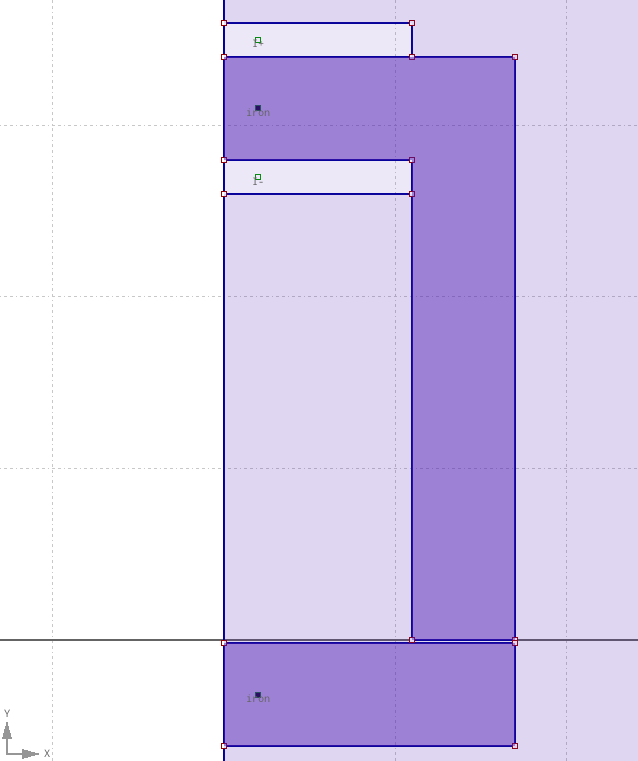
\includegraphics[width=0.7\columnwidth]{../assets/assignment_1_geometry.png}}
\caption{Simulationsgeometrie in der ersten Aufgabenstellung; $I = 64\ A$.}
\label{assignment_1_geometry}
\end{figure}

\begin{figure}
\centerline{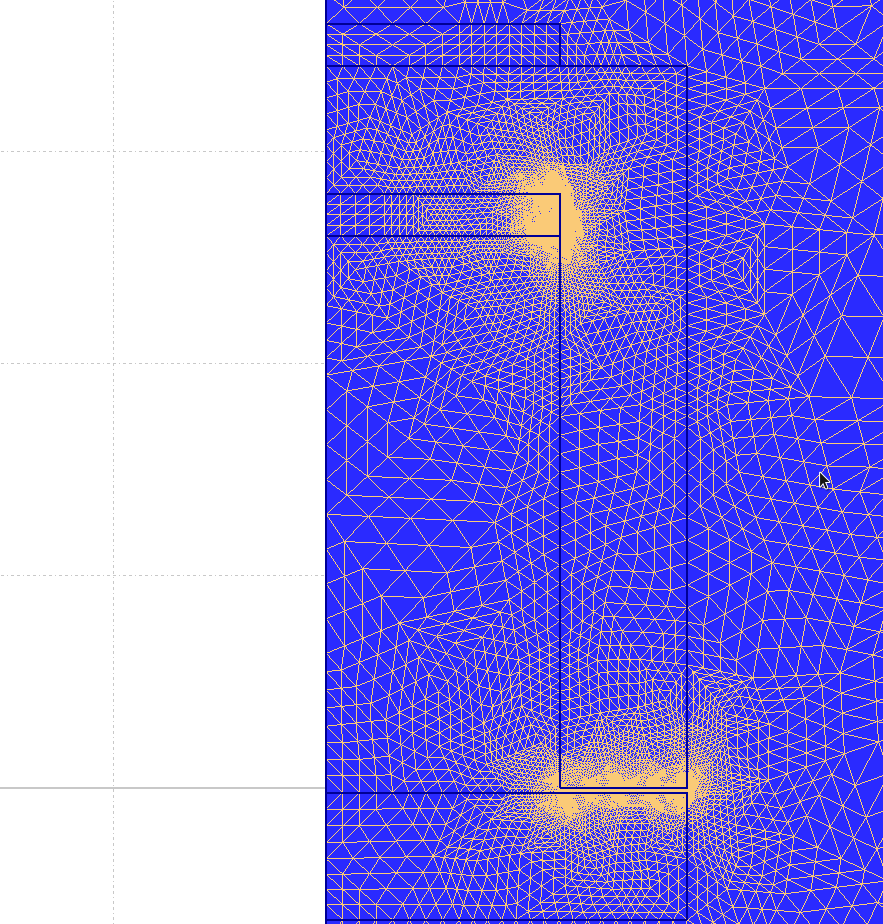
\includegraphics[width=0.7\columnwidth]{../assets/assignment_1_mesh.png}}
\caption{Simulationsvermaschung in der ersten Aufgabenstellung; $I = 64\ A$.}
\label{assignment_1_mesh}
\end{figure}

\begin{figure}
\centerline{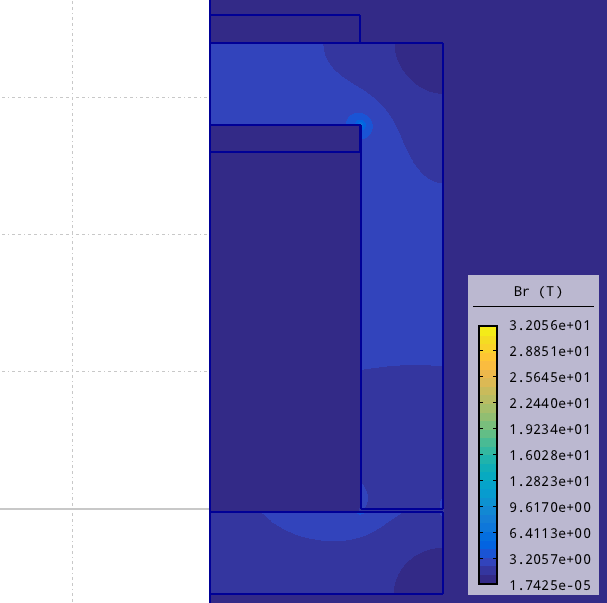
\includegraphics[width=0.7\columnwidth]{../assets/assignment_1_simulation.png}}
\caption{Flussdichteverteilung in der ersten Aufgabenstellung; $I = 64\ A$.}
\label{assignment_1_simulation}
\end{figure}

\begin{figure}
\centerline{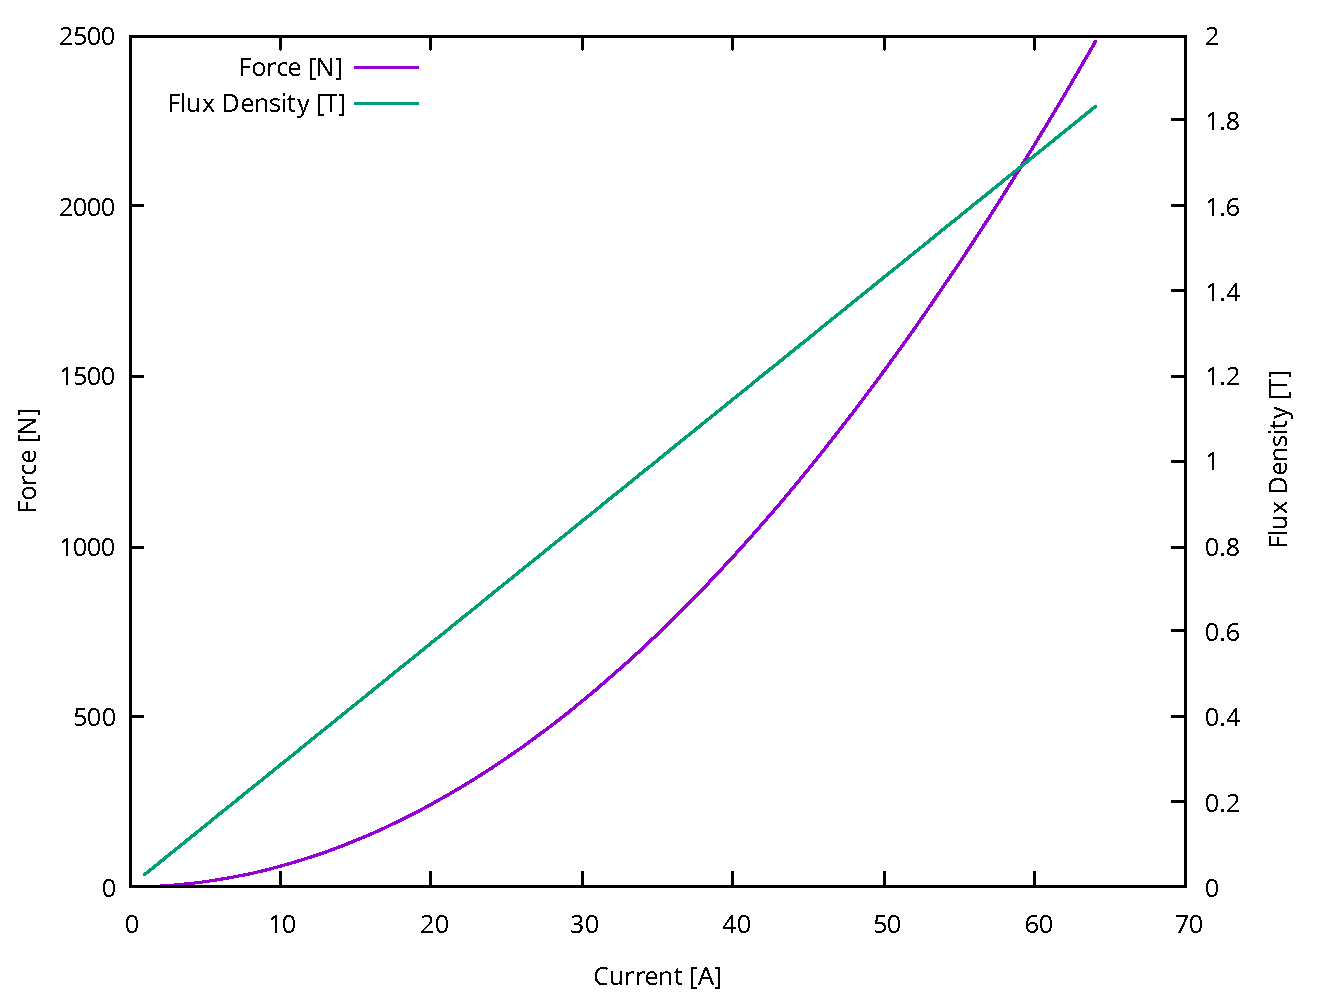
\includegraphics[width=\columnwidth]{../assets/assignment_1_plot.pdf}}
\caption{Kraft auf das I-Joch und Flussdichte im Luftspalt gegenüber Stromstärke.}
\label{assignment_1_plot}
\end{figure}

Für den in Projekt 2 zunächst simulierten Strom von $16\ A$ ergab sich dort eine Kraft auf das I-Joch von $162,96\ N$ (Aufgabe I.C.). Abweichend dazu ergab sich in dieser Simulation eine Kraft von $155,09\ N$, was einer Abweichung von etwa $4,8\ \%$ entspricht, der Wert liegt also in der erwarteten Größenordnung. Die beobachtete Abweichung kommt möglicherweise durch eine leicht andere Simulationsgeometrie (runde vs. rechteckige Randbegrenzung, andere Dimensionen der Spule) zustande, außerdem konnte kein Weg gefunden werden, wie in Projekt 2 die Sollfläche der Polygone per Skript zu begrenzen.

Abb.~\ref{assignment_1_plot} zeigt einen Plot der Kraft auf das I-Joch und Flussdichte im Luftspalt für Ströme von $1\ A$ bis $64\ A$. Die bereits in Projekt 2, Aufgabe I.D. geäußerte Vermutung, dass $F \sim I²$ zeigt sich bestätigt. Für die Flussdichte im Lufspalt zeigt sich ein Zusammenhang $B \sim I$. Dies deckt sich mit dem aus der Physik bekannten Wissen, dass sich die mag. Flussdichte B einer Spule mit Länge l, Windungszahl N, Strom I und Kernmaterial mit $\mu_0$ durch

\begin{equation}
B = \mu_0 \cdot \mu_r \cdot {N \cdot I \over l}
\label{eq_magnetic_field_coil}
\end{equation}

beschreiben lässt.

Für die Kraft auf eine von der Flussdichte B durchflossene Grenzfläche A des magnetischen Kreises gilt dann

\begin{equation}
F = {1 \over 2} \cdot {B² \over \mu_0} \cdot A
\label{eq_electromagnetic_force}
\end{equation}

Die analytische Beschreibung des vorliegenden Problems entspricht also qualitativ dem beobachteten Simulationsergebnis.

\section{Aufgabenstellung 2}

Für die zweite Aufgabenstellung wird der Strom in der Spule zu Null gesetzt und der untere Teil des U-Joches durch ein permanentmagnetisches Material mit $\mu_r = 1,11$ und der Remanenzflussdichte $B = 1,28\ T$ ersetzt, welches im der parametrischen Modellgenerierung mit variabler Dicke erstellt werden kann. Zunächst wird eine Dicke von $3\ mm$ betrachtet, anschließend eine variable Dicke von $1 - 11\ mm$.

Dargestellt ist beispeilhaft eine Dicke d von $11\ mm$. Abb.~\ref{assignment_2_geometry} zeigt die Simulationsgeometrie, Abb.~\ref{assignment_2_mesh} das generierte Netz und Abb.~\ref{assignment_2_simulation} die resultierende Flussdichteverteilung. Die Netzknotenanzahl betrug in diesem Fall 22162; die Anzahl der Polygone 37168.

\begin{figure}
\centerline{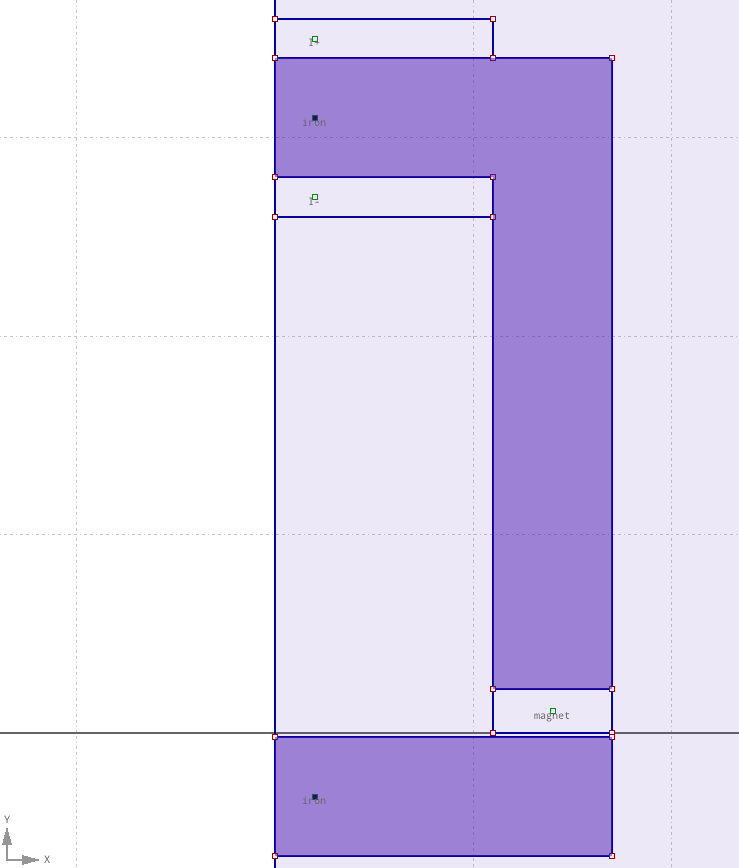
\includegraphics[width=0.7\columnwidth]{../assets/assignment_2_geometry.png}}
\caption{Simulationsgeometrie in der zweiten Aufgabenstellung; $d = 11\ mm$.}
\label{assignment_2_geometry}
\end{figure}

\begin{figure}
\centerline{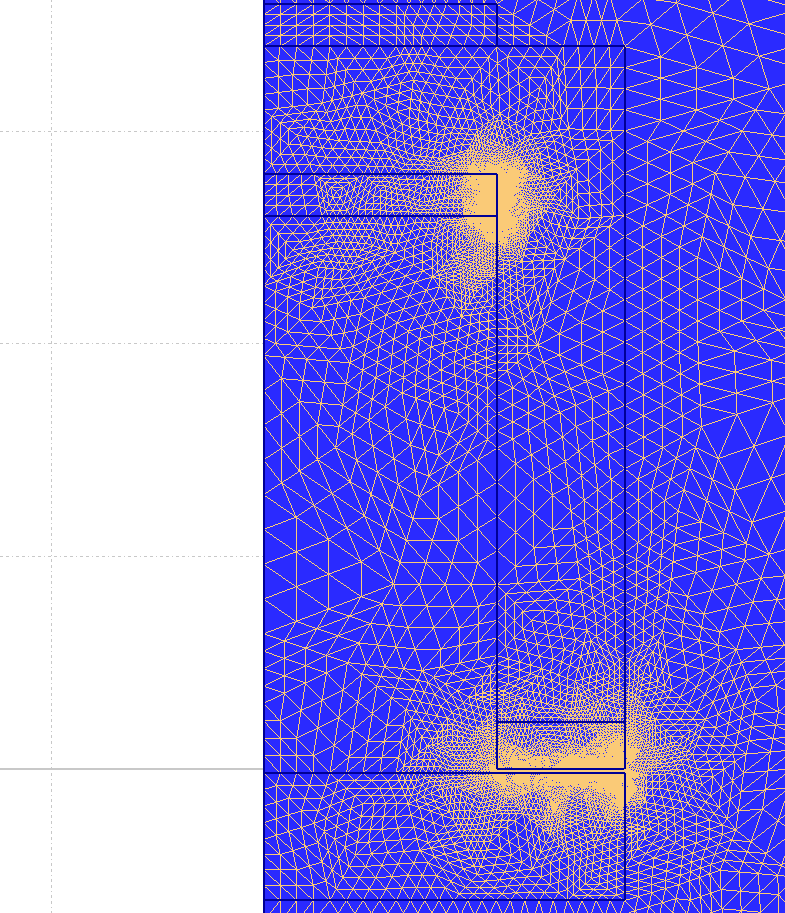
\includegraphics[width=0.7\columnwidth]{../assets/assignment_2_mesh.png}}
\caption{Simulationsvermaschung in der zweiten Aufgabenstellung; $d = 11\ mm$.}
\label{assignment_2_mesh}
\end{figure}

\begin{figure}
\centerline{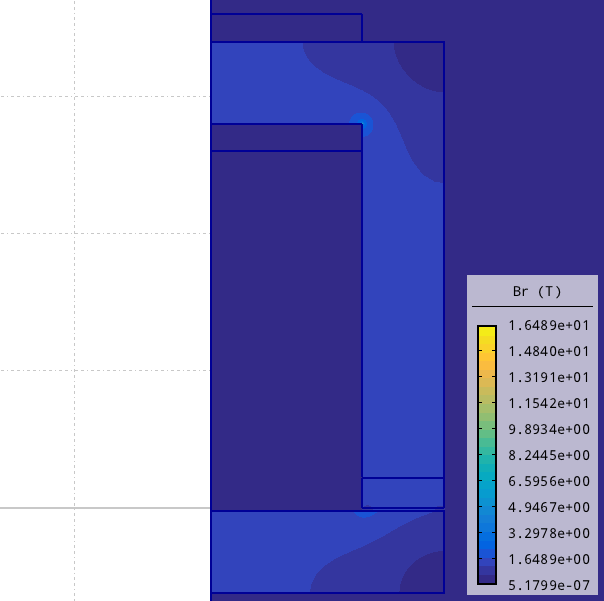
\includegraphics[width=0.7\columnwidth]{../assets/assignment_2_simulation.png}}
\caption{Flussdichteverteilung in der zweiten Aufgabenstellung; $d = 11\ mm$.}
\label{assignment_2_simulation}
\end{figure}

\begin{figure}
\centerline{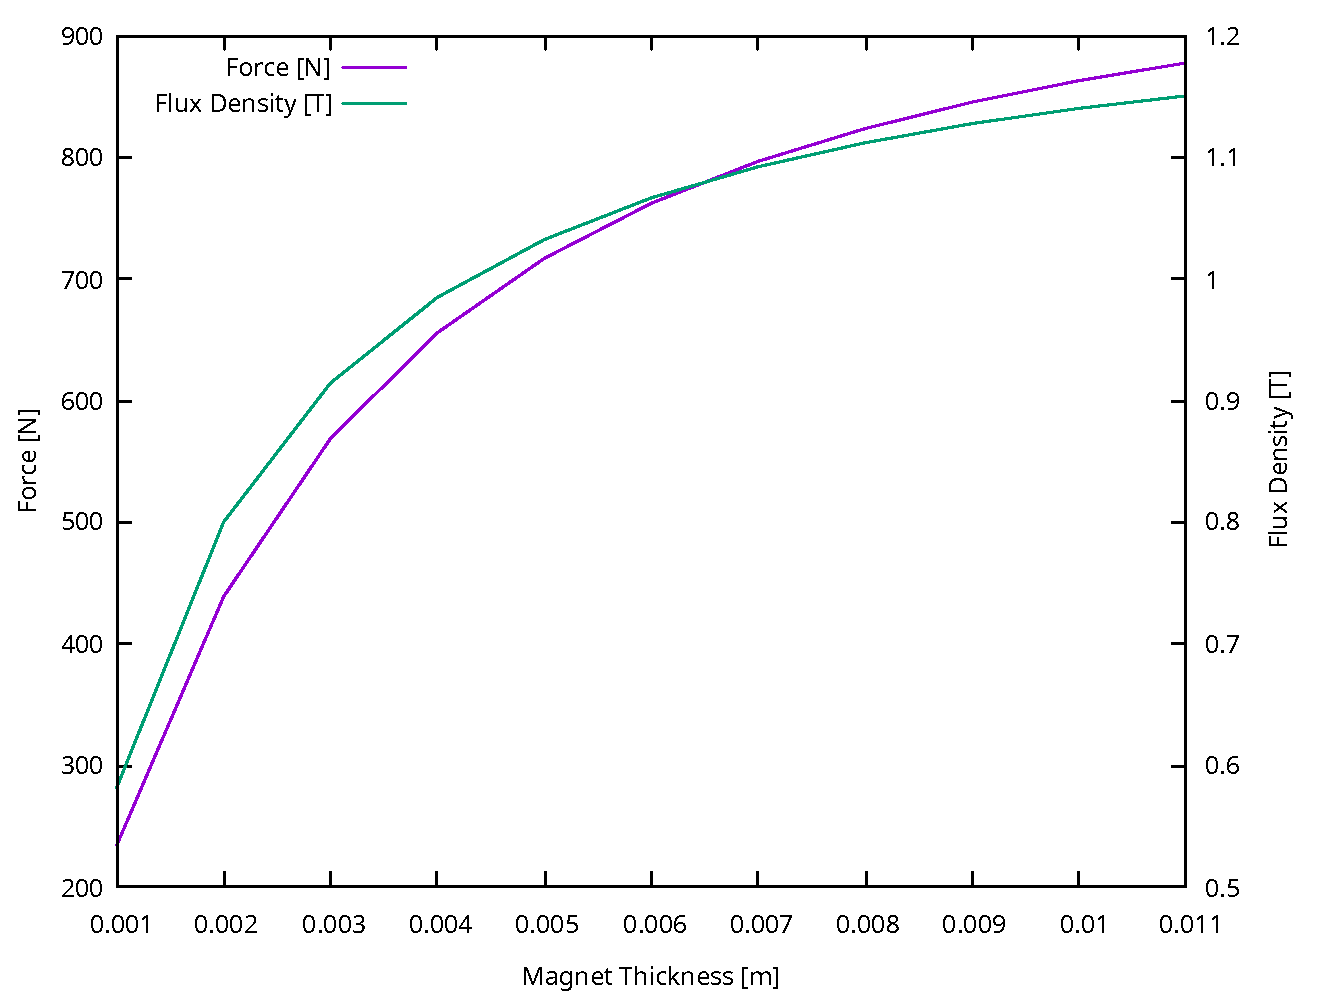
\includegraphics[width=\columnwidth]{../assets/assignment_2_plot.pdf}}
\caption{Kraft auf das I-Joch und Flussdichte im Luftspalt gegenüber Dicke des Permanentmagneten.}
\label{assignment_2_plot}
\end{figure}

Für eine Dicke $d = 3\ mm$ des permanentmagnetischen Material ergibt sich eine Anziehungskraft $F = 568,69\ N$ sowie eine Flussdichte im Spalt $B = 0,914\ T$.

Da in diesem Projekt nicht mit Magnetisierungskurven und auch sonst mit leicht anderen Werten gearbeitet wurde, ist kein direkter Vergleich der Werte mit den ensprechenden aus Projekt 2, Aufgabe II.B. möglich.

Bei Betrachtung des Verlaufs der Kraft auf das I-Joch und Flussdichte im Luftspalt für Dicken von $1\ mm$ bis $11\ mm$ in Abb.~\ref{assignment_2_plot} zeigt sich jedoch qualitativ das gleiche Verhalten wie in Projekt 2; auch hier strebt die Flussdichte und nach Gl.~(\ref{eq_electromagnetic_force}) die Kraft asymptotisch gegen ein Maximum.

Dieses Verhalten ergibt sich aus der Hysterese des ferromagnetischen Material des Permanentmagneten, dass durch die Angabe der Remanenzflussdichte in der Simulation angegeben wurde. Hierdurch bedingt gerät das Material in eine magnetische Sättigung, in der eine Erhöhung der magnetischen Feldstärke H nicht mehr linear eine Erhöhung der magnetischen Flussdichte bewirkt.

\section{Aufgabenstellung 3}

In der dritten Aufgabenstellung werden die in den vorheringen beiden Aufgabenstellungen betrachteten Probleme kombiniert, in dem die Dicke des permanentmagnetischen Materials zu 3 mm gesetzt wird und die Spule mit einem variablen Strom von $I = -60 .. 60\ A$ beaufschlagt wird.

Dargestellt ist beispeilhaft ein Strom von $60\ A$. Abb.~\ref{assignment_3_geometry} zeigt die Simulationsgeometrie, Abb.~\ref{assignment_3_mesh} das generierte Netz und Abb.~\ref{assignment_3_simulation} die resultierende Flussdichteverteilung. Die Netzknotenanzahl betrug in diesem Fall 20936; die Anzahl der Polygone 35120.

\begin{figure}
\centerline{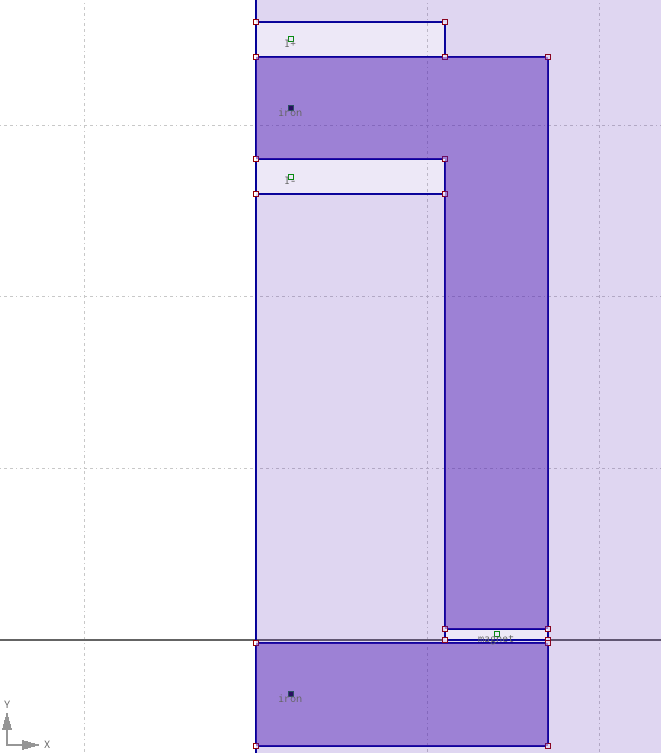
\includegraphics[width=0.7\columnwidth]{../assets/assignment_3_geometry.png}}
\caption{Simulationsgeometrie in der dritten Aufgabenstellung; $I = 60\ A$.}
\label{assignment_3_geometry}
\end{figure}

\begin{figure}
\centerline{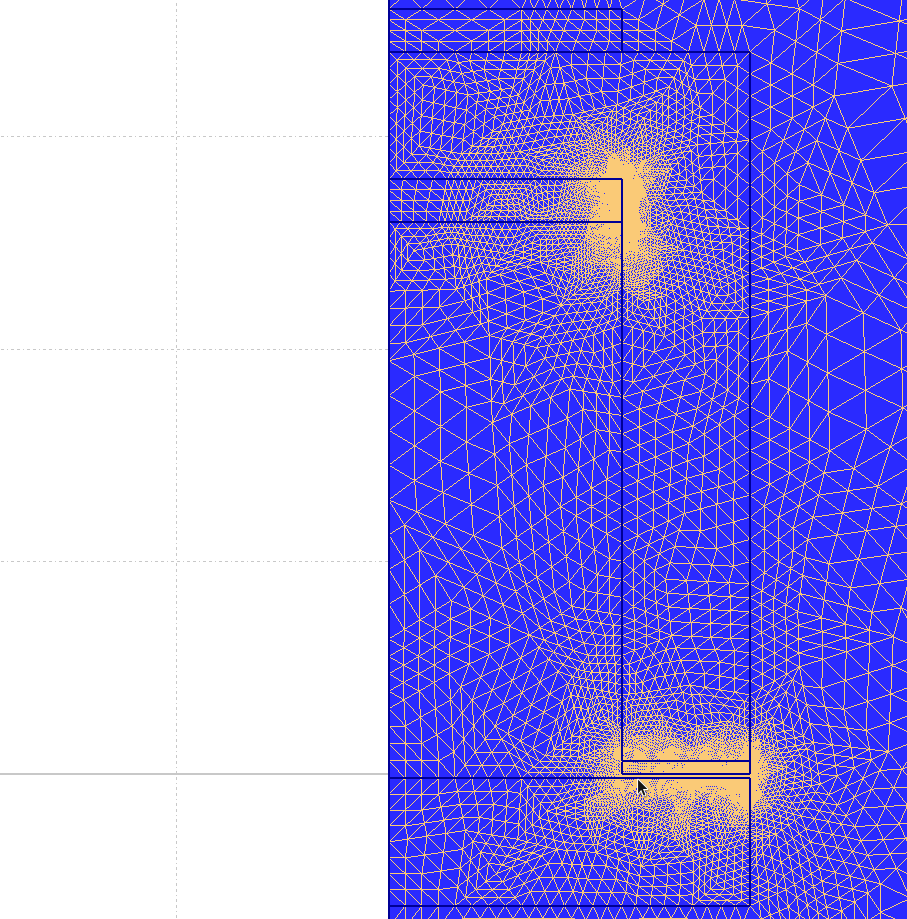
\includegraphics[width=0.7\columnwidth]{../assets/assignment_3_mesh.png}}
\caption{Simulationsvermaschung in der dritten Aufgabenstellung; $I = 60\ A$..}
\label{assignment_3_mesh}
\end{figure}

\begin{figure}
\centerline{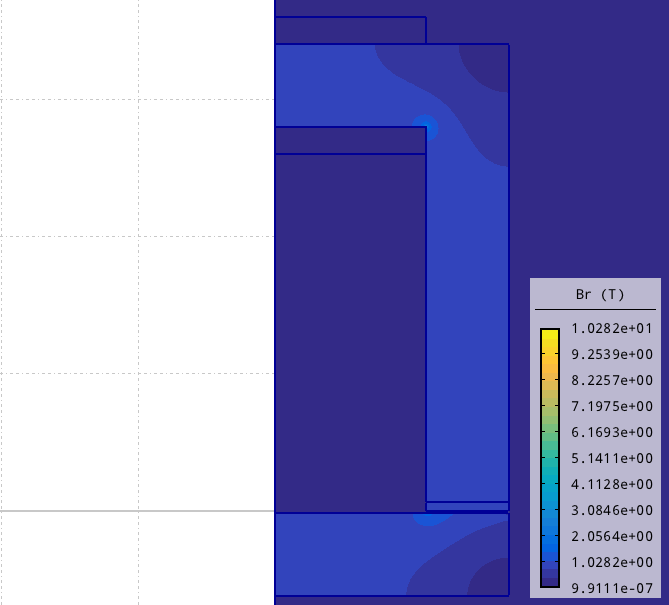
\includegraphics[width=0.7\columnwidth]{../assets/assignment_3_simulation.png}}
\caption{Flussdichteverteilung in der dritten Aufgabenstellung; $I = 60\ A$..}
\label{assignment_3_simulation}
\end{figure}

\begin{figure}
\centerline{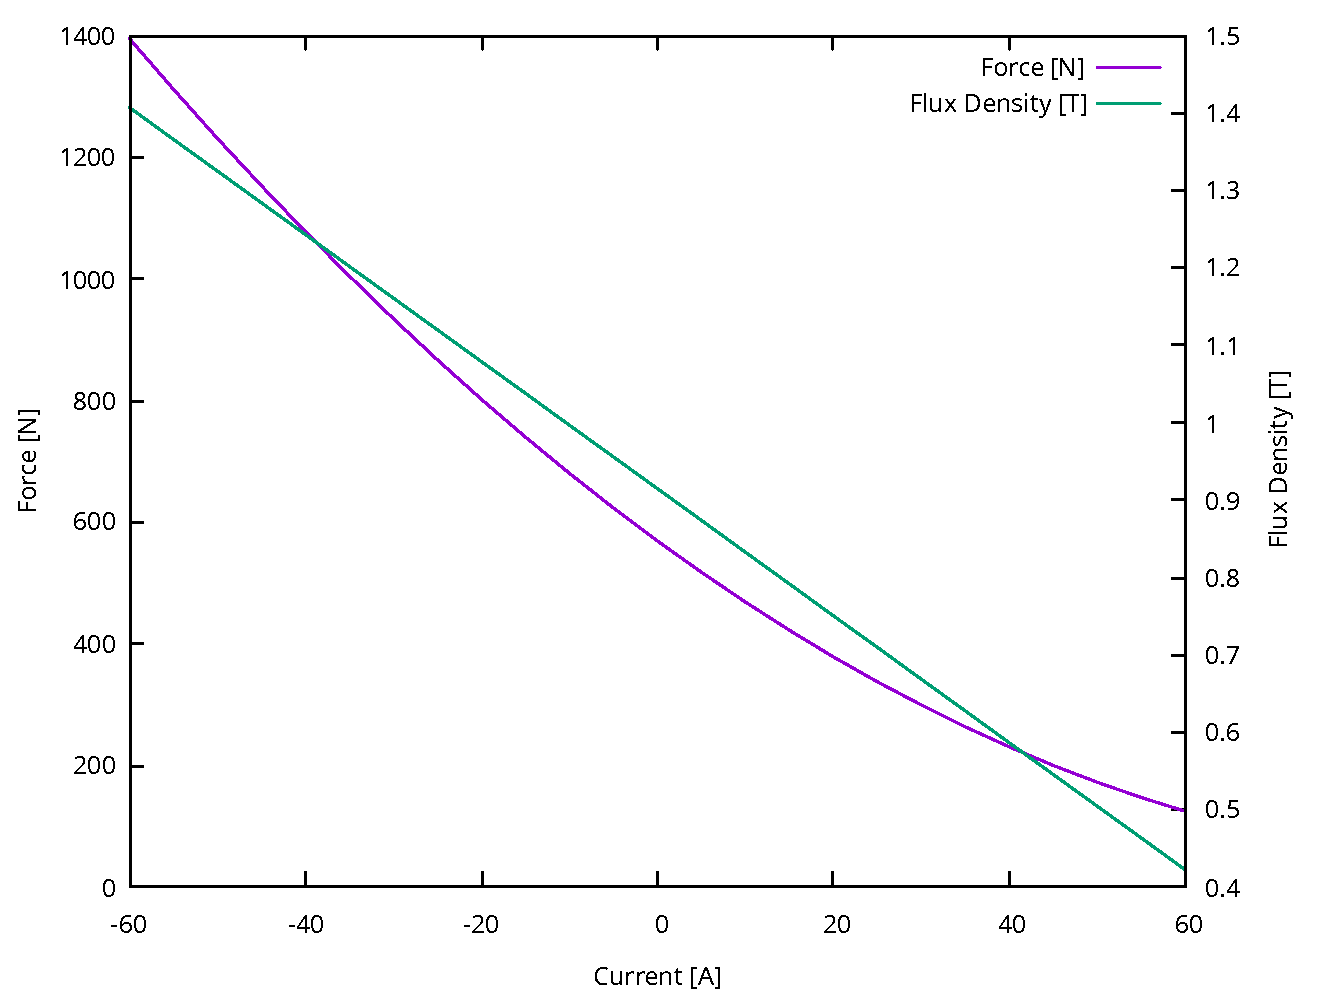
\includegraphics[width=\columnwidth]{../assets/assignment_3_plot.pdf}}
\caption{Kraft auf das I-Joch und Flussdichte im Luftspalt gegenüber Stromvorgabe.}
\label{assignment_3_plot}
\end{figure}

Bevor die beobachteten Simulationsergebnisse diskutiert werden, sollen noch einmal die Ergebnisse aus Aufgabenstellung 1 und 2 rekapituliert und eine Hypothese für das Verhalten in dieser Simulation formuliert werden.

In Aufgabenstellung 1 wurde beobachtet, dass sich für größere Ströme im betrachteten und zwischen den Simulationen nicht veränderten, nicht-invertierten Drehsinn der Spule (positiver Strom oben, negativer unten) eine linear größer werdende Feldstärke einstellt, die nach Gl.~(\ref{eq_electromagnetic_force}) eine quadratisch größer werdende Kraft zur Folge hat. Da Gleichung Gl.~(\ref{eq_electromagnetic_force}) in den betrachteten Fällen immer gilt, und die Anziehungskraft der Flussdichte direkt zuordnet, soll in der weiteren Betrachtung eine Reduktion auf die Betrachtung der Flussdichte erfolgen. Bei einem Strom von $0\ A$ herrscht eine Flussdichte von $0\ T$; bei einem Strom von $60\ A$ eine Flussdichte von $1,72\ T$.

In Aufgabenstellung 2 konnte beobachtet werden, dass für größere Dicken des permanentmagnetischen Materials eine Sättigung der aufgebrachten magnetischen Flussdichte eintritt. Einer Dicke des Permanentmagneten von $3\ mm$ konnte hier eine Flussdichte von $0,91\ T$ ermittelt werden.

Werden nun beide Effekte überlagert betrachtet, so kann vermutet werden, dass sich die beiden Flussdichten addieren. Da als Ergebnissgröße der Simulation nur der Betrag des resultierenden B-Feld-Vektors betrachtet wird, kann nicht direkt geschlossen werden, wie die Überlagerung der beiden Felder im Lufspalt vektoriell erfolgt. Eine weitere Schlussfolgerung ist, dass ein komplett "linearer" Verlauf des B-Feldes nicht vorliegen kann, da ein solcher durch die Betragsbildung in eine Betragsfunktion umgewandelt werden würde. Wäre in Aufgabenstellung 1 eine Simulation auch für negative Ströme erfolgt, so hätte sich gezeigt, dass das resultierende Flussdichte eine Betragsfunktion um $0\ A$ ergeben hätte. Ein Überlagern mit einem anderen konstanten Feld führt nun zu einer Linearverschiebung des B-Felds, die sich nach der Betragsbildung in einer Verschiebung der "Spitze" der Betragsfunktion äußert. Es kann somit also Bereiche geben, in denen eine Erhöhung des Stroms zu einer Verringerung der Flussdichte führt.

Das Simulationsergebnis in Abb.~\ref{assignment_3_plot} bestätigt diese Hypothese. Es zeigt sich, dass die Flussdichte für größer werdende Ströme linear abfällt. Für einen Strom von $0\ A$ stellt sich ein erwartetes Magnetfeld von $0,91\ T$ ein. Bei einem Strom von $60\ A$ beträgt das Magnetfeld $0,42\ T$, was nahe legt, dass die Überlagerung nicht antiparallel erfolgt.

\begin{figure}
\centerline{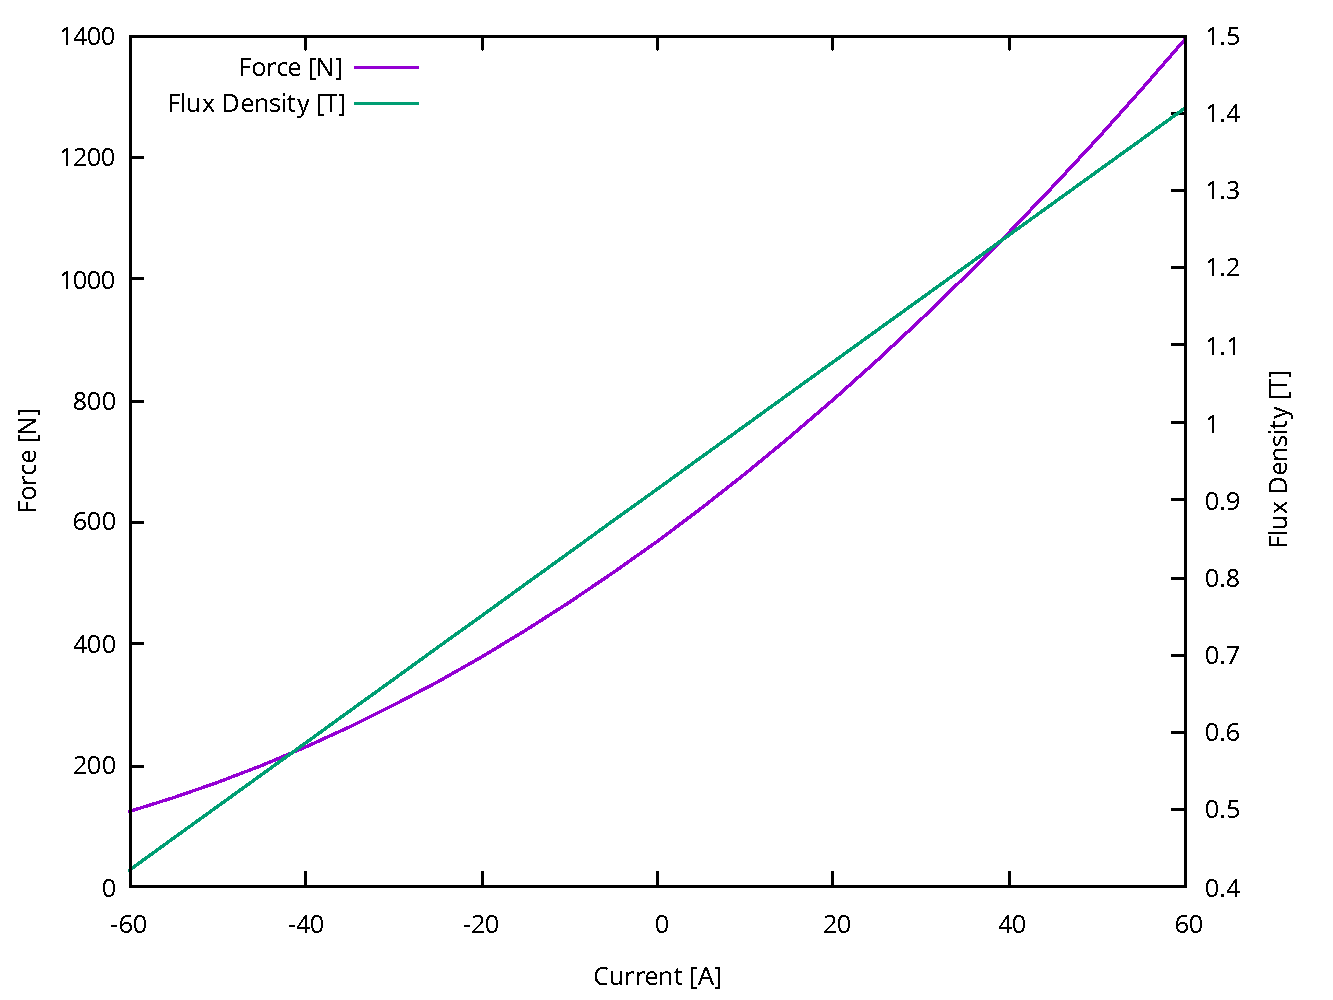
\includegraphics[width=\columnwidth]{../assets/assignment_3_plot_swapped_polarity.pdf}}
\caption{Kraft auf das I-Joch und Flussdichte im Luftspalt bei invertiertem Spulendrehsinn.}
\label{assignment_3_plot_swapped_polarity}
\end{figure}

\begin{figure}
\centerline{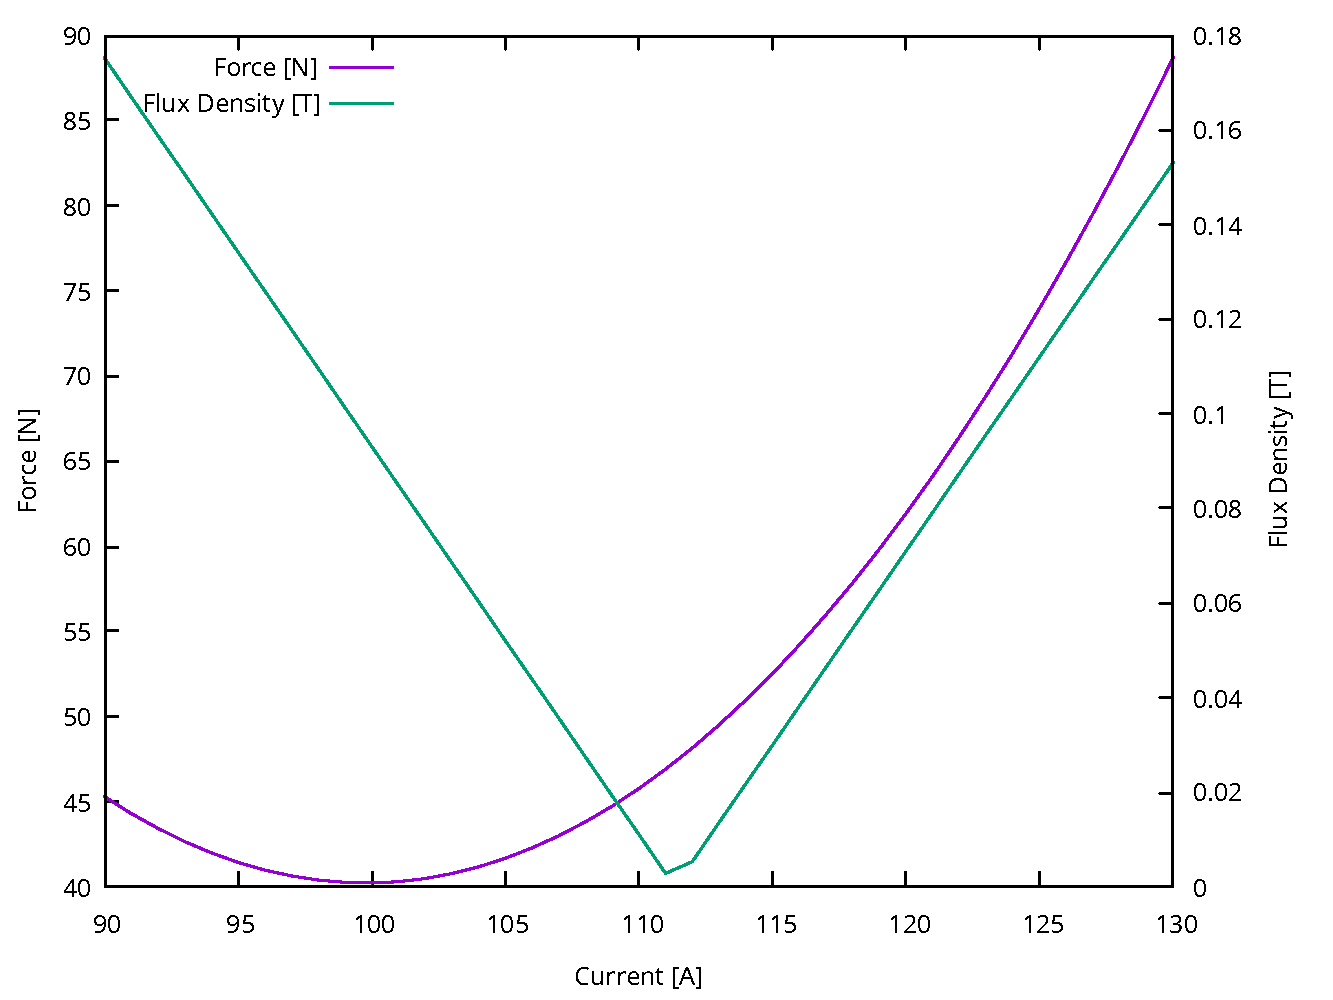
\includegraphics[width=\columnwidth]{../assets/assignment_3_plot_zero.pdf}}
\caption{Kraft auf das I-Joch und Flussdichte im Luftspalt in der Nähe des Nullpunktes der Flussdichte.}
\label{assignment_3_plot_zero}
\end{figure}

Wird der Drehsinn der Spule invertiert, überlagern sich die B-Felder im betrachteten Bereich des Stromes konstruktiv additiv, da das Minimum der Flussdichte nun in die andere Richtung verschoben ist (Abb.~\ref{assignment_3_plot_swapped_polarity}).

Der Punkt, an dem die Flussdichte ihr Minimum hat, soll genauer untersucht werden. Dazu wird (mit normalem Drehsinn der Spule) der Strombereich von $90 - 130\ A$ simuliert (Abb.~\ref{assignment_3_plot_zero}). Dieser Punkt wird bei ca. $111,5\ A$ erreicht. Auffällig ist jedoch, dass in der Nähe dieses Punktes Gl.~(\ref{eq_electromagnetic_force}) verletzt wird. Nach Ihrer Definition verwunder dies jedoch nicht, da dort zur Kraftberechnung ein homogenes magnetisches Feld über die wirksame Fläche angenommen wird. Bedingt durch Randeffekte ist dies eine Vereinfachung, die in diesem Grenzfall versagt.

Abschließend soll noch einmal auf die in Aufgabenstellung 2 getroffenen Aussagen zu Sättigungseffekten des permanentmagnetischen Materials eigegangen werden, die ja offenbar in dieser Aufgabestellung nicht eintreten. Dies lässt sich darauf zurückführen, dass in der Simulation lediglich eine Remanenzflussdichte angegeben wurde, also die maximale Flussdichte, die das Material als Permanentmagnet aufbringen kann. Dies ist eine unvollstängige Beschreibung, die die Sättigungseffekte durch extern aufgebrachte Felder außer acht lässt. Für eine Korrekte Betrachtung hätte eine Magnetisierungskennlinie wie in Projekt 2 mit angegeben werden müssen. Die simulierte Ergebnisse würden sich also für ein echt eingebrachtes ferromagnetisches Material nicht wie in dieser Simulation einstellen.

\end{document}
